\apendice{Documentación técnica de programación}

\section{Introducción}
Este apéndice proporciona una guía detallada sobre la estructura del código del proyecto, las herramientas usadas para el funcionamiento de la aplicación junto con su configuración.
Se analiza la estructura de directorios que hay en la aplicación, además se incluye un manual del programador en el que se explica cómo instalar y configurar el entorno de desarrollo junto con la ejecución del proyecto.
Con este apéndice se intenta que futuros desarrolladores que vayan a modificar o mejorar la aplicación sepan cómo dejar todo instalado y configurado de la mejor forma posible.

\section{Estructura de directorios}

El proyecto \textbf{GreenInHouse 2.0} sigue una estructura de directorios bien organizada, permitiendo una gestión eficiente del código, los recursos y la configuración. A continuación, se describen las principales carpetas y su contenido:

\begin{itemize}
    \item {\textbf{Directorio raíz} (\texttt{greeninhouse2/})}
    Este es el directorio principal del proyecto y contiene archivos de configuración esenciales para Flutter y Dart, además de la estructura del código fuente.

    \begin{itemize}
    \item \textbf{\texttt{.dart\_tool/}}: Carpeta generada automáticamente por Flutter y Dart con herramientas internas necesarias para la compilación.
    \item \textbf{\texttt{.idea/}}: Archivos de configuración de Android Studio para la organización del proyecto.
    \item \textbf{\texttt{build/}}: Carpeta generada durante la compilación, almacena archivos de salida del proyecto.
    \item \textbf{\texttt{ios/}, \texttt{android/}, \texttt{linux/}, \texttt{macos/}, \texttt{web/}, \texttt{windows/}}: Carpetas para cada plataforma soportada, con la configuración y código necesarios para compilar en cada sistema operativo.

    \item \texttt{\textbf{assets}/} Carpeta con todas las fotos que se van a usar en la aplicación.
    \item \textbf{\texttt{flags/}}: Carpeta con imágenes de iconos y estados de las plantas:

    \item{\texttt{\textbf{lib/}}}
    Directorio principal del código fuente en Flutter. Aquí se encuentra la lógica de la aplicación.
    \begin{itemize}
    \item \textbf{\texttt{generated/}}: Contiene archivos generados automáticamente para la internacionalización.
    \begin{itemize}
        \item \texttt{intl/l10n.dart} – Configuración de localización.
    \end{itemize}
    \item \textbf{\texttt{l10n/}}: Dedicada a la internacionalización del proyecto.
    \begin{itemize}
        \item \texttt{intl\_en.arb} – Traducciones en inglés.
        \item \texttt{intl\_es.arb} – Traducciones en español.
    \end{itemize}

    \item \textbf{\texttt{api\_service.dart}} – Implementación de las llamadas a la API.
    \item \textbf{\texttt{botones\_inicio.dart}} – Definición de la barra de navegación inferior.
    \item \textbf{\texttt{main.dart}} – Punto de entrada principal de la aplicación.

    \item \texttt{\textbf{pantalla\_graficas.dart}} – Pantalla principal con gráficos de sensores.
    \item \texttt{\textbf{pantalla\_inicio.dart}} – Pantalla inicial de la aplicación.
    \item \texttt{\textbf{pantalla\_comprobacion\_sensores.dart}} – Revisión del estado de sensores.
    \item \texttt{\textbf{pantalla\_creacionplantas.dart}} – Creación de nuevas plantas.
    \item \texttt{\textbf{pantalla\_modificarplanta.dart}} – Modificación de plantas registradas.
    \item \texttt{\textbf{pantalla\_eliminarplanta.dart}} – Eliminación de plantas registradas.

    \item \texttt{\textbf{grafica\_humedad.dart}} – Representación de datos de humedad.
    \item \texttt{\textbf{grafica\_luz.dart}} – Visualización de datos de luminosidad.
    \item \texttt{\textbf{grafica\_temperatura.dart}} – Evolución de la temperatura.
    \end{itemize}

    \item \texttt{\textbf{.gitignore}} – Definición de archivos y carpetas a excluir del repositorio Git.
    \item \texttt{.metadata} – Archivo interno de configuración de Flutter.
    \item \texttt{\textbf{analysis\_options.yaml}} – Reglas de análisis de código en Dart.
    \item \texttt{\textbf{greeninhouse2.iml}} – Configuración de IntelliJ/Android Studio.
    \item \texttt{\textbf{pubspec.yaml}} – Definición de dependencias, assets e información del proyecto.
    \item \texttt{\textbf{pubspec.lock}} – Registro de versiones de las dependencias utilizadas.
    \item \texttt{\textbf{README.md}} – Documentación inicial sobre el proyecto y su instalación.
    \end{itemize}
\end{itemize}

\section{Manual del programador}
El objetivo del manual del programador es proporcionar una guía del desarrollo y mantenimiento de la aplicación. Este manual está dirigido a desarrolladores que necesiten saber cómo funcionan las herramientas utilizadas en el desarrollo de esta aplicación.
También se han incluido las instrucciones necesarias para configurar el entorno de desarrollo y ejecutar la aplicación.
Además, se han detallado aspectos que son clave, como la estructura de datos que sigue la aplicación y la comunicación con la API, entre otras cosas, con el objetivo de facilitar mejoras que se puedan llevar a cabo en un futuro.


\subsection{\textbf{Instalación de Android Studio}}
Android Studio es el entorno de desarrollo integrado (IDE) oficial que se usa en el desarrollo de \textit{apps} para Android. Basado en el potente editor de código y las herramientas para desarrolladores de IntelliJ IDEA.
Se puede descargar desde su página oficial \cite{AndroidStudio}.




Al descargar la aplicación y ejecutarla, nos saldrá lo que vemos en la figura \ref{C1} a continuación y le daremos al botón de ``Next''.
\begin{figure}[H]
    \centering
    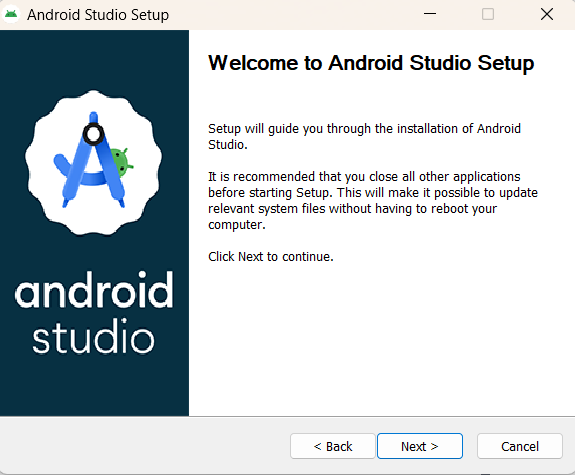
\includegraphics[width=0.8\linewidth]{AndroidStudio1.png}
    \caption{Primer paso de la instalación de Android Studio.}
    \label{C1}
\end{figure}

Tras esto nos saldrá la ventana \ref{C2} en la que dejaremos lo que viene por defecto y le volveremos a dar a ``Next''.
\begin{figure}[H]
    \centering
    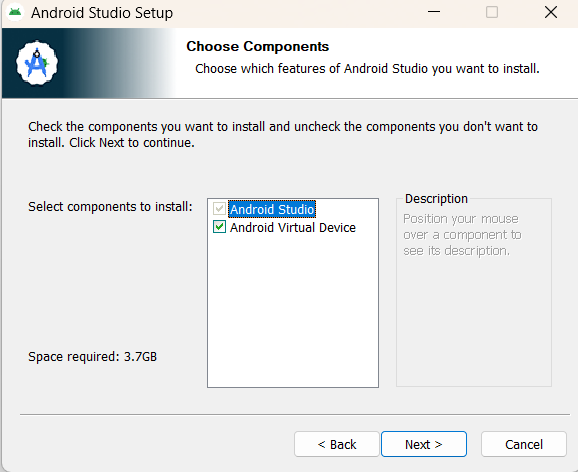
\includegraphics[width=0.8\linewidth]{AndroidStudio2.png}
    \caption{Segundo paso de la instalación de Android Studio.}
    \label{C2}
\end{figure}

Por último, decidiremos la ruta donde instalar la aplicación, como se puede ver en la figura \ref{C3} y le daremos a ``Next'' para que instale la aplicación en la ruta seleccionada.
\begin{figure}[H]
    \centering
    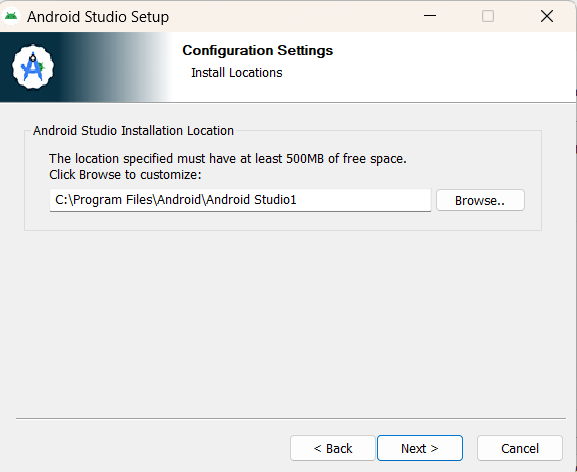
\includegraphics[width=0.8\linewidth]{AndroidStudio3.png}
    \caption{Ruta de la instalación}
    \label{C3}
\end{figure}

Tras instalar Android Studio, vamos a pasar a la configuración de las herramientas instalando tanto Flutter como Dart.
Esto se hace entrando en la pestaña de ajustes y en Plugins, como vemos en la figura\ref{C4}.

\begin{figure}[H]
    \centering
    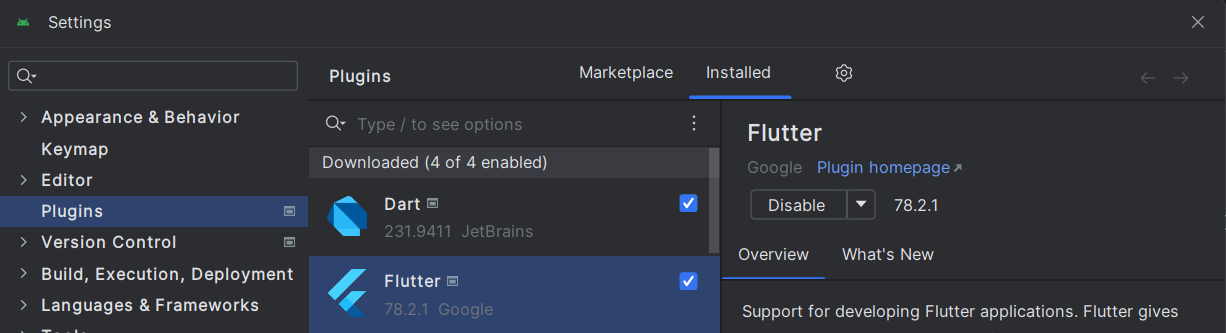
\includegraphics[width=0.8\linewidth]{PlugingsAndroidStudio.png}
    \caption{Instalación plugins Android Studio}
    \label{C4}
\end{figure}


El siguiente paso es la configuración de SDK en el Android Studio. Esto se hace accediendo a ajustes y allí desde Languages \& Frameworks como vemos en la figura \ref{C5}.

\begin{figure}[H]
    \centering
    \includegraphics[width=0.8\linewidth]{Configuración-SDK-AndroidStudio.png}
    \caption{Configuración de SDK en Android Studio}
    \label{C5}
\end{figure}


Por último, vamos a instalar unas herramientas en SDK Tools que vienen a la derecha de la de SDK Platforms, como vemos en la figura \ref{C6}, necesarias para el buen funcionamiento de la herramienta.

\begin{figure}[H]
    \centering
    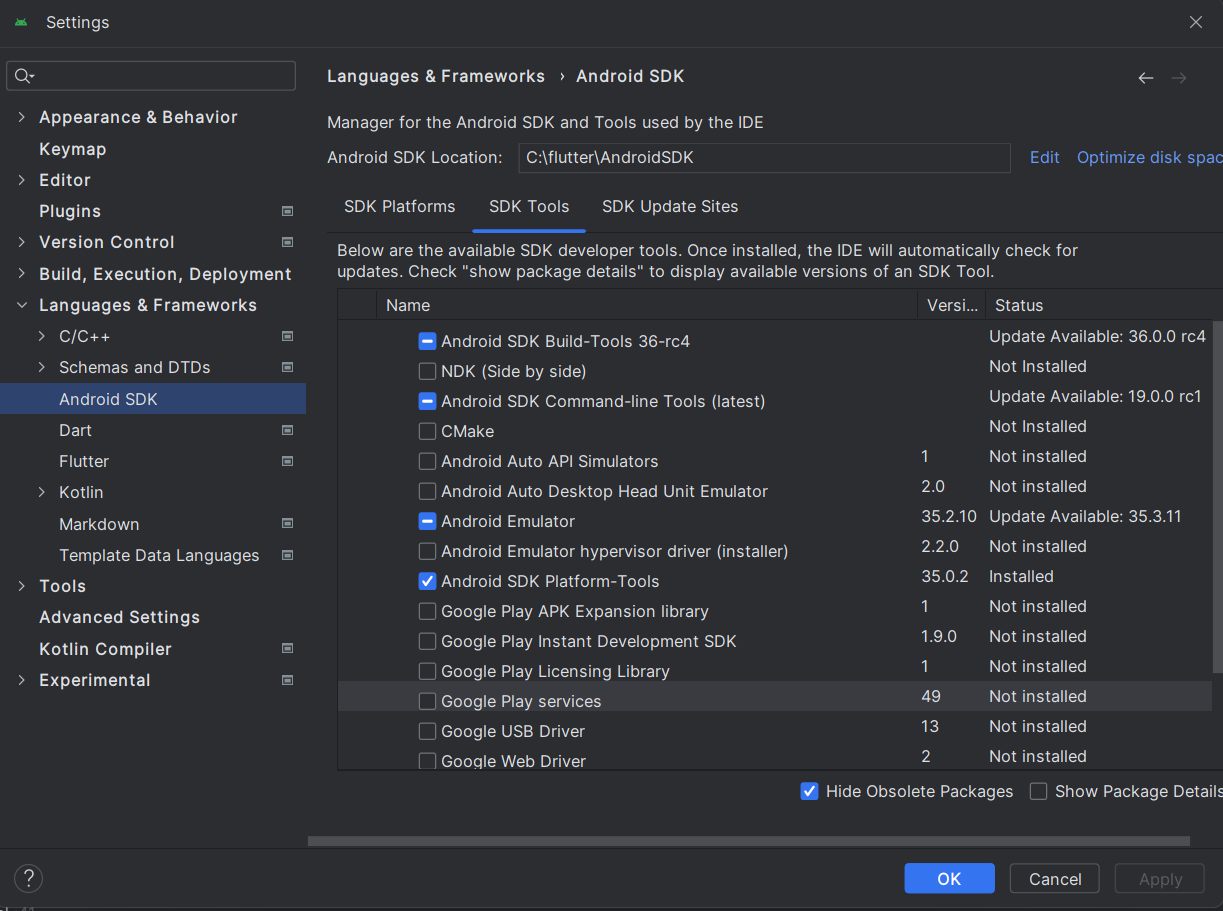
\includegraphics[width=0.8\linewidth]{Configuracion-SDKTools-AndroidStudio.png}
    \caption{Instalación de Herramientas de SDK}
    \label{C6}
\end{figure}

\subsection{\textbf{Instalación de Flutter}}
Para la instalación de Flutter tendremos que ir a su página web \cite{Flutter} y descargarlo. Allí nos preguntarán por nuestro sistema operativo, tras elegirlo nos preguntarán por el tipo de aplicación que queremos ya sea ``Android'' o ``Web'' o ``Desktop''. En este caso, se selecciona ``Windows'' y ``Android''. Tras esto, nos descargaremos el .zip que aparece en la web, como se puede ver en la figura \ref{C7}.

\begin{figure}[H]
    \centering
    \includegraphics[width=0.8\linewidth]{Instalación_Flutter_SDK.png}
    \caption{Descarga del archivo.}
    \label{C7}
\end{figure}

A continuación, deberemos descomprimir el .zip y guardar la carpeta en un directorio que elijamos para de esta manera poder añadir en las variables de entorno la ruta del fichero ``\textbackslash bin''.

Primero, abriremos la configuración avanzada del sistema desde el buscador de Windows y nos saldrá la pantalla que vemos en la figura \ref{C8}. Daremos al botón que pone ``Variables de entorno'' para continuar.

\begin{figure}[H]
    \centering
    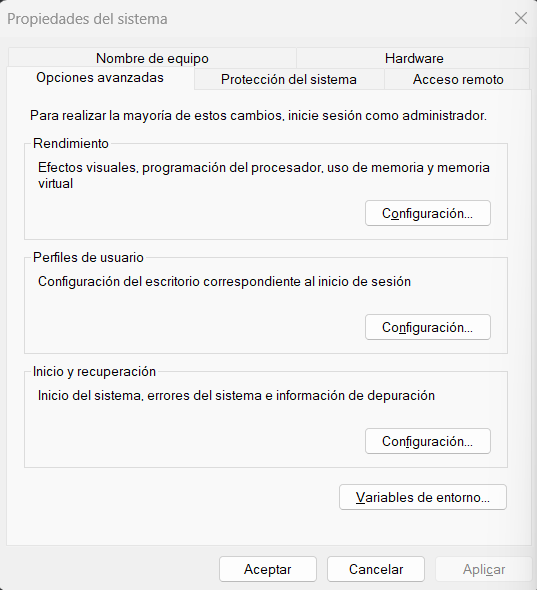
\includegraphics[width=0.8\linewidth]{Variables_Entorno_1.png}
    \caption{Pantalla de configuración avanzada.}
    \label{C8}
\end{figure}

Seguido, buscaremos la variable que se llame ``Path'' y le daremos al botón de ``Editar'' como vemos en la figura \ref{C9}.

\begin{figure}[H]
    \centering
    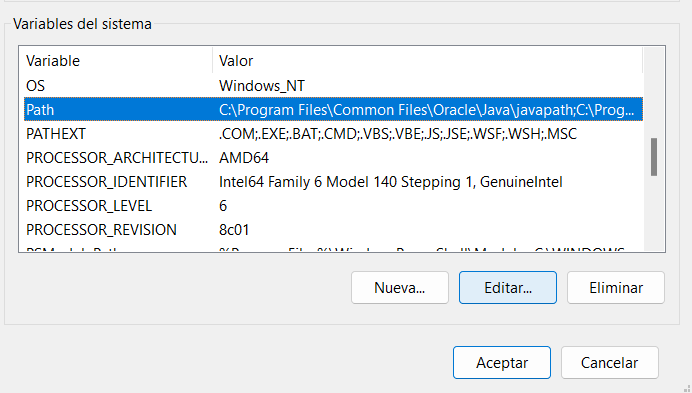
\includegraphics[width=0.8\linewidth]{Variables_Entorno_2.png}
    \caption{Pantalla de variables de entorno.}
    \label{C9}
\end{figure}

Por último, le daremos al botón de ``Nuevo'' y añadiremos la ruta donde se encuentre nuestra carpeta ``\textbackslash bin''. Nos quedará añadido, como se puede ver en la figura \ref{C10} y le daremos a ``Aceptar'' para que se quede guardado.

\begin{figure}[H]
    \centering
    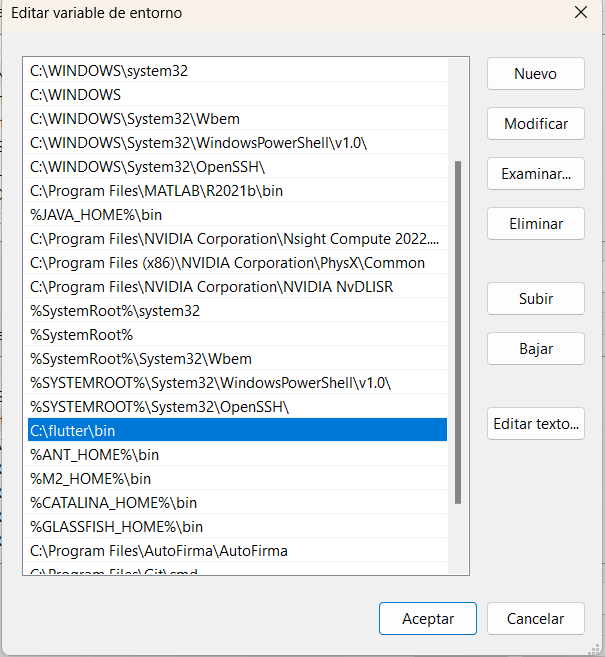
\includegraphics[width=0.8\linewidth]{Variables_Entorno_3.png}
    \caption{Pantalla de editar variables de entorno.}
    \label{C10}
\end{figure}

Para comprobar que todo se ha instalado correctamente, abriremos una terminal y, mediante el comando \textit{``flutter doctor''} verificaremos que se ha instalado bien y si falta alguna configuración o dependencia, como podemos ver en la figura \ref{C11}.

\begin{figure}[H]
    \centering
    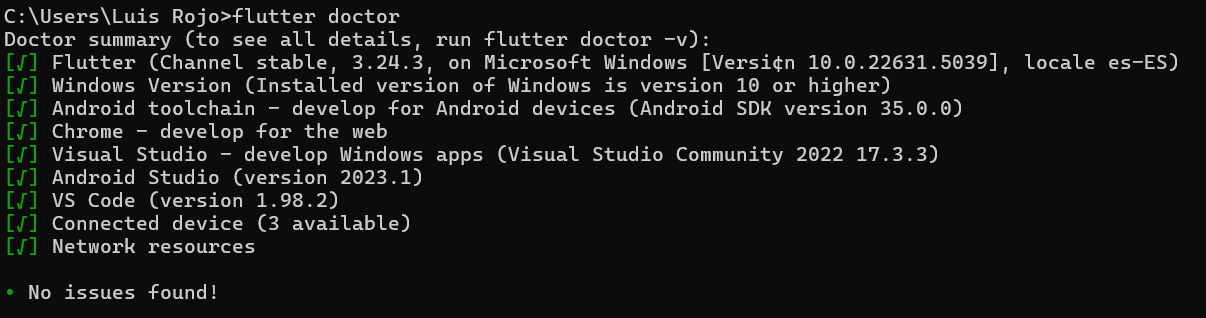
\includegraphics[width=0.8\linewidth]{Comando_flutterdoctor.png}
    \caption{Uso del comando \textit{``flutter doctor''}}
    \label{C11}
\end{figure}

\section{Compilación, instalación y ejecución del proyecto}

Para poder probar y utilizar la aplicación de GreenInHouse 2.0 durante su desarrollo ha sido necesario el uso de un emulador. El propio AndroidStudio tiene sus propios emuladores, los cuales puedes descargar y configurar en función de tus intereses de la aplicación.

Para poder llevar a cabo la ejecución del programa primero deberemos descargarnos el proyecto mediante el uso del comando:
\texttt{git clone https://github.com/LuisRojoSanz/GreenInHouse2\_APP.git}

Tras esto se habrá descargado el contenido del repositorio de github y se podrá ejecutar el proyecto.

Primero se deberá pulsar el botón del ``+'' en \textit{Device Manager} para empezar a descargar el emulador como se ve en la figura \ref{C12}.

\begin{figure}[H]
    \centering
    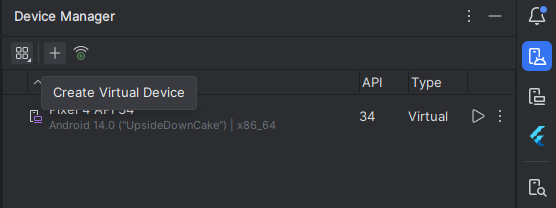
\includegraphics[width=0.8\linewidth]{InstalacionyEjecucion1.png}
    \caption{Descarga de un emulador}
    \label{C12}
\end{figure}

Una vez se haya pulsado el ``+'' aparecerá la ventana que vemos en la figura \ref{C13} en la que se seleccionará el modelo de emulador deseado y se pulsará el botón ``Next''.

\begin{figure}[H]
    \centering
    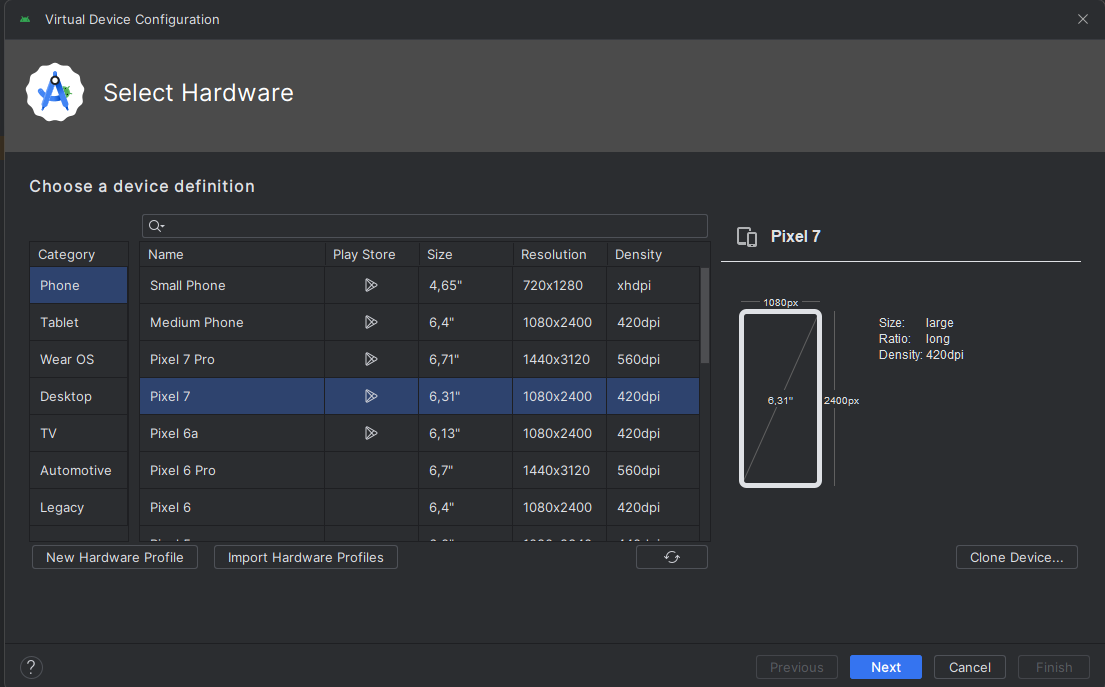
\includegraphics[width=0.8\linewidth]{InstalacionyEjecucion2.png}
    \caption{Seleccionando un emulador}
    \label{C13}
\end{figure}

Tras esto habrá que seleccionar la versión de Android que vemos en la figura \ref{C14} o una superior para el correcto funcionamiento del proyecto y darle al botón de ``Next''

\begin{figure}[H]
    \centering
    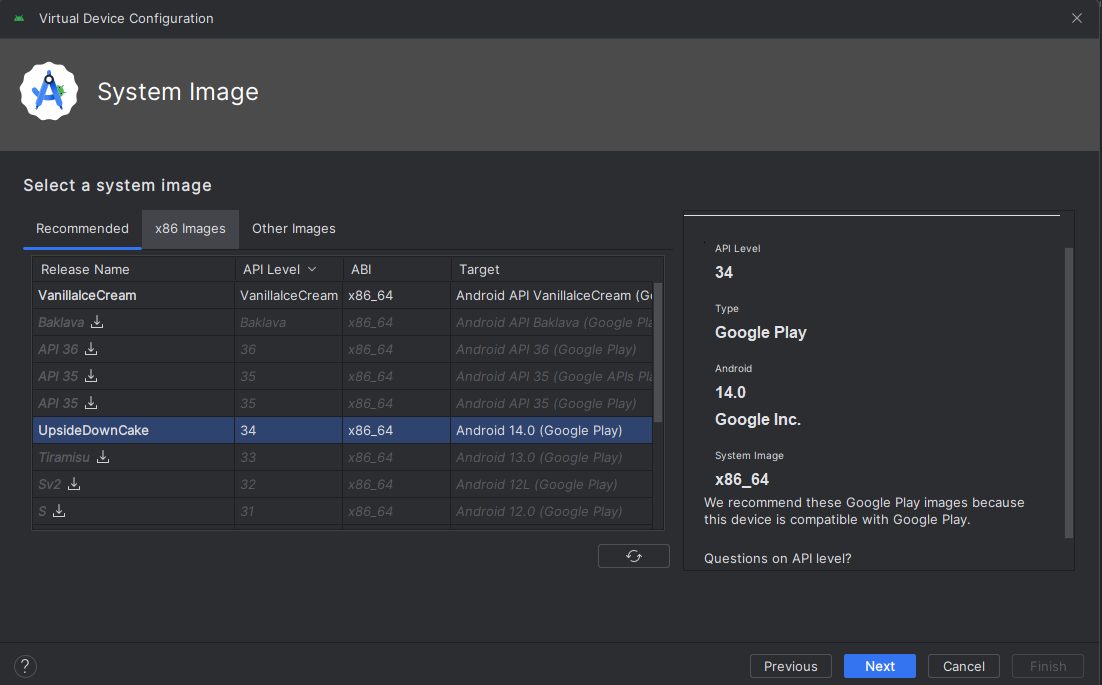
\includegraphics[width=0.8\linewidth]{InstalacionyEjecucion3.png}
    \caption{Seleccionando la versión de Android del emulador}
    \label{C14}
\end{figure}

En la pantalla que vemos en la figura \ref{C15} se deberá verificar la configuración del emulador y seleccionar el nombre que se desee. Una vez verificado, se dará al botón de ``Next''.

\begin{figure}[H]
    \centering
    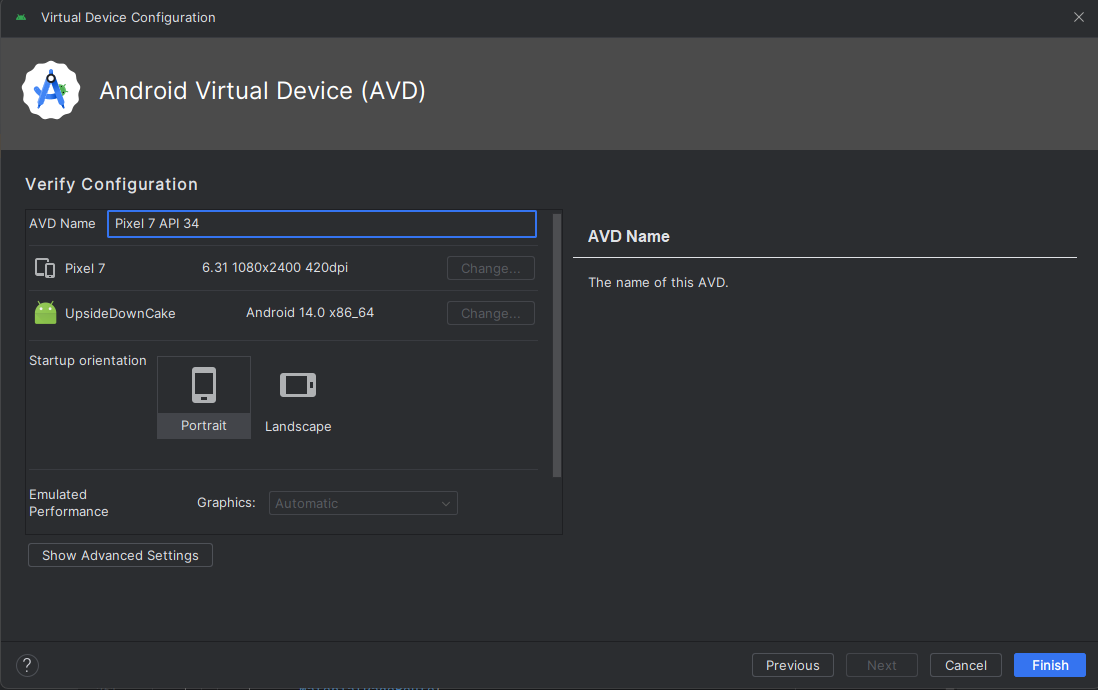
\includegraphics[width=0.8\linewidth]{InstalacionyEjecucion4.png}
    \caption{Verificar la configuración del emulador}
    \label{C15}
\end{figure}

Descargado ya el emulador, tocará seleccionarlo como se muestra en la figura \ref{C16} resaltado en azul. Una vez seleccionado, se empezará a ejecutar el emulador.

\begin{figure}[H]
    \centering
    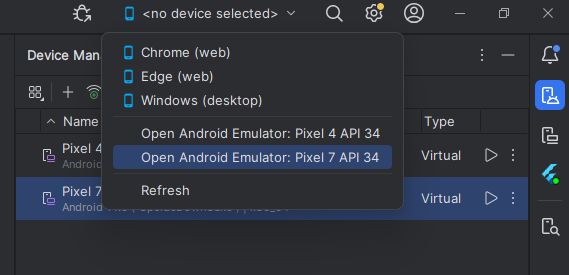
\includegraphics[width=0.8\linewidth]{InstalacionyEjecucion5.png}
    \caption{Ejecución del emulador}
    \label{C16}
\end{figure}

Por último, una vez que el emulador ya ha iniciado, como vemos en la figura \ref{C17}, se deberá pulsar el botón verde de ejecutar de arriba a la izquierda que está rodeado en azul. Una vez pulsemos este botón, se comenzará a ejecutar el proyecto.

\begin{figure}[H]
    \centering
    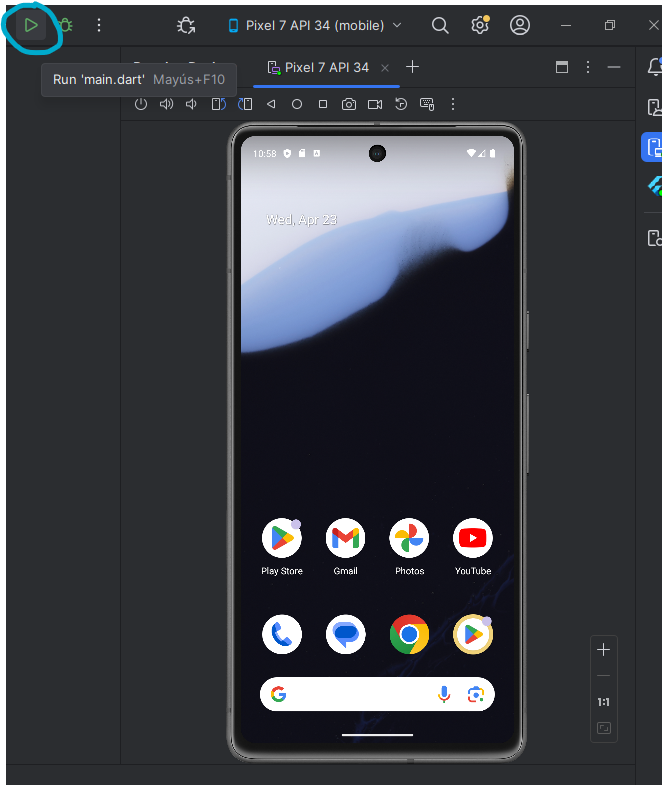
\includegraphics[width=0.8\linewidth]{InstalacionyEjecucion6.png}
    \caption{Ejecución del proyecto}
    \label{C17}
\end{figure}


\section{Pruebas del sistema}
Para garantizar que la aplicación GreenInHouse 2.0 funciona de manera correcta, se han llevado a cabo diferentes tipos de pruebas: 

\subsection{Pruebas Funcionales:} Estas pruebas se basan en comprobar que cada una de las funcionalidades de los requisitos funciona de manera correcta, como por ejemplo:
    \begin{enumerate}
        \item \textbf{Crear Planta:} El sistema permite que el usuario pueda seleccionar el nombre y tipo de planta y crear la planta.
        \item \textbf{Consultar Hitos}: La comunicación con la base de datos a través de la API hace que se puedan ver los hitos diarios.
        \item \textbf{Cambiar Idioma:} El usuario selecciona el idioma que desee y automáticamente se cambia el idioma en toda la aplicación.
        \item \textbf{Seleccionar Imagen de Planta:} El usuario puede sacar una foto con la cámara o seleccionarla de la galería.
    \end{enumerate}
\subsection{Pruebas de Integración:} Estas pruebas se realizan comprobando la comunicación entre la aplicación y la base de datos mediante diferentes peticiones HTTP dentro de la red local. Estas peticiones pueden ser:
    \begin{enumerate}
        \item \textbf{GET:} Mediante esta llamada se realizan las solicitudes de lectura a la API como pueden ser la obtención del estado de los sensores.
        \item \textbf{POST:} Mediante esta llamada se realizan las solicitudes a la API para la creación de nuevos datos en la base de datos, como puede ser la creación de una nueva planta.
        \item \textbf{PUT:} Mediante esta llamada se realizan las solicitudes a la API para la modificación de datos ya creados, como puede ser la modificación del tipo de planta.
        \item \textbf{DELETE:} Mediante esta llamada se realizan las solicitudes a la API para la eliminación de datos creados en la API, como puede ser la eliminación de una planta.
    \end{enumerate}
\subsection{Pruebas de Interfaz de Usuario:} Este tipo de pruebas se basan en el correcto funcionamiento de la interfaz de usuario, como puede ser:
    \begin{enumerate}
        \item \textbf{Funcionamiento de botones y demás \textit{widgets}:} Se han hecho pruebas para comprobar que tanto los botones como los demás elementos con los que puede interactuar el usuario de la interfaz funcionen de manera correcta.
        \item \textbf{Adaptabilidad:} Se han hecho pruebas para comprobar que usando teléfonos móviles de diferentes resoluciones la interfaz se adapta de manera correcta.
    \end{enumerate}
\subsection{Pruebas de robustez:}
Se han hecho también pruebas simulando fallos para ver cómo reaccionaba la aplicación. Este tipo de pruebas han sido, por ejemplo:
    \begin{enumerate}
        \item \textbf{Sin conexión a internet:} Se han hecho pruebas pruebas para ver cómo reaccionaba la aplicación en caso de que no hubiera conexión a internet y por tanto no se pudiera comunicar la aplicación con la API. Se ha observado que la aplicación sigue funcionando solo que no ofrece dichos servicios que necesitan de los datos de la base de datos.
        \item \textbf{Plantas con el mismo nombre:} Se han hecho pruebas intentando crear una planta con el mismo nombre que otra ya existente. Al intentar esta prueba la aplicación ha dado error debido a la existencia de una planta con ese mismo nombre.
    \end{enumerate}
    